%!TEX root = advanced.tex

\section{Strukturierung}

\subsection{Abbildungen und Verweise}

\livecoding{Abbildungen und Verweise}

\subsection{Titelseite}

\begin{frame}
  \begin{center}
    \begin{tikzpicture}
      \node[fill=white,blur shadow,inner sep=0pt,draw=gray,very thin] {
        \pgfimage[height=.95\paperheight]{demo/thesis-titlepage}
      };
    \end{tikzpicture}
  \end{center}
\end{frame}

\begin{frame}[fragile]{Schriftarten manuell umschalten}
  Ein Dokument besitzt
  \begin{itemize}
    \item \textsf{eine serifenlose Schriftfamilie}\newline
      (zum Beispiel für Überschriften)\newline
      Verwendung durch \lstinline-\textrm- oder \lstinline-\rmfamily-
    \item \textrm{eine Schriftfamilie mit Serifen}\newline
      (zum Beispiel für den Fließtext)\newline
      Verwendung durch \lstinline-\textsf- oder \lstinline-\sffamily-
    \item \texttt{eine nichtproportionale Schriftfamilie}\newline
      (zum Beispiel für Quelltext)\newline
      Verwendung durch \lstinline-\texttt- oder \lstinline-\ttfamily-
  \end{itemize}

  \xxx

  \begin{exampleblock}{Andere Schriftarten}
    \begin{itemize}
      \item Computer Modern ist Standard
      \item \lstinline-\usepackage{lmodern}- lädt Latin Modern
      \item Pakete für viele andere Schriftarten vorhanden
    \end{itemize}
  \end{exampleblock}
\end{frame}

\begin{frame}[fragile]{Schriftgrößen manuell umschalten}
  \begin{center}
    \tiny \lstinline-\tiny-

    \scriptsize \lstinline-\scriptsize-

    \footnotesize \lstinline-\footnotesize-

    \small \lstinline-\small-

    \normalsize \lstinline-\normalsize-

    \large \lstinline-\large-

    \Large \lstinline-\Large-

    \LARGE \lstinline-\LARGE-

    \huge \lstinline-\huge-

    \Huge \lstinline-\Huge-
  \end{center}

  \normalsize
\end{frame}

\begin{frame}[fragile]{Abstände manuell ergänzen}
  \begin{itemize}
    \item \lstinline-\vspace{1cm}-, \lstinline-\hspace{1cm}-\newline
      für zusätzlichen \alert{v}ertikalen oder \alert{h}orizontalen Abstand
    \item \lstinline-\vfill-, \lstinline-\hfill-\newline
      für flexiblen Abstand, sodass Seite voll wird
  \end{itemize}

  \xxx

  \begin{alertblock}{Achtung}
    \begin{itemize}
      \item Nur sinnvoll auf Titelseiten oder Folien.
      \item In Dokumenten macht \LaTeX\ das besser als Du!
    \end{itemize}
  \end{alertblock}
\end{frame}

\livecoding{Quelltext der Titleseite}

\subsection{Kopf- und Fußzeilen}

\begin{frame}[fragile]{Seitenstile}{Wieviel Kopf- und Fußzeile darf es sein?}
  \begin{block}{In der Präambel}
    \begin{lstlisting}[gobble=6,style=block]
      \usepackage{scrpage2}
      \pagestyle{scrheadings}
    \end{lstlisting}
  \end{block}

  \vskip1ex

  \begin{tabular}{r@{ }l}
    \lstinline-empty- & keine Kopf- und keine Fußzeile \\
      & (automatisch auf Titelseite) \\[1ex]
    \lstinline-scrplain- & wenig Kopf- und Fußzeile \\
      & (automatisch auf erster Seite eines Kapitels) \\[1ex]
    \lstinline-scrheadings- & normale Kopf- und Fußzeile \\
      & (automatisch auf normalen Seiten)
  \end{tabular}

  \vskip1ex

  \begin{block}{Seitenstil manuell wechseln}
    \begin{lstlisting}[gobble=6,style=block]
      \pagestyle{empty} % ab jetzt
      \thispagestyle{empty} % nur für diese Seite
    \end{lstlisting}
  \end{block}
\end{frame}

\begin{frame}[fragile,t]{Kolumnentitel}{Automatische Kolumnentitel}
  \xxx\xxx

  \begin{Definition}[Lebende Kolumnentitel]
    Textabhängige Informationen in der Kopfzeile.\\
    Zum Beispiel aktuelles Kapitel und aktueller Abschnitt.
  \end{Definition}

  \xxx

  \begin{lstlisting}[gobble=4]
    \automark[section]{chapter}
  \end{lstlisting}
  \begin{itemize}
    \item Kapitel auf linken/geraden Seiten
    \item Abschnitt auf rechten/ungeraden Seiten
  \end{itemize}

  Mögliche Werte sind dabei: \lstinline-part-, \lstinline-chapter-,
  \lstinline-section-, \lstinline-subsection-.
\end{frame}

\begin{frame}[fragile,t]{Kolumnentitel}{Manuelle Kolumnentitel}
  \xxx\xxx

  \only<presentation>{
    \begin{Definition}[Lebende Kolumnentitel]
      Textabhängige Informationen in der Kopfzeile.\\
      Zum Beispiel aktuelles Kapitel und aktueller Abschnitt.
    \end{Definition}
  }

  \xxx

  \begin{lstlisting}[gobble=4]
    \manualmark % Automatik aus
    \markboth{linke Seite}{rechte Seite}
    % oder nur
    \markright{rechte Seite}
  \end{lstlisting}
\end{frame}

\mode
<article>

\begin{frame}[fragile]{Kolumnentitel}{Manuelle Automatik}
  \begin{lstlisting}[gobble=4]
    \manualmark % Automatik aus
    \renewcommand{\chaptermark}[1]{%
      \markboth{Kapitel \thechapter\ #1}{}}
    \renewcommand{\sectionmark}[1]{%
      \markboth{Abschnitt \thesection\ #1}{}}
  \end{lstlisting}
  \lstinline-\chaptermark- wird von \LaTeX\ mit Beginn
  jeden neuen Kapitels mit dem Namen des Kapitels aufgerufen.
\end{frame}

\mode
<all>

\begin{frame}[fragile]{Befehle zur Konfiguration des Seitenstils}
  \begin{tikzpicture}[
      node distance=9mm,
      on grid
    ]
    \draw[maincolor,very thick,dashed]
      (1,0) -- (5,0) -- (5,6) -- (1,6) -- cycle
      (-1,0) -- (-5,0) -- (-5,6) -- (-1,6) -- cycle;

    \node[inner sep=0pt,minimum width=1cm,minimum height=5mm,fill=maincolor]
      at (-4.25,5.5) (lehead) {};
    \node[inner sep=0pt,minimum width=1cm,minimum height=5mm,fill=maincolor]
      at (-3,5.5) (cehead) {};
    \node[inner sep=0pt,minimum width=1cm,minimum height=5mm,fill=maincolor]
      at (-1.75,5.5) (rehead) {};

    \node[inner sep=0pt,minimum width=1cm,minimum height=5mm,fill=maincolor]
      at (-4.25,.5) (lefoot) {};
    \node[inner sep=0pt,minimum width=1cm,minimum height=5mm,fill=maincolor]
      at (-3,.5) (cefoot) {};
    \node[inner sep=0pt,minimum width=1cm,minimum height=5mm,fill=maincolor]
      at (-1.75,.5) (refoot) {};

    \node[inner sep=0pt,minimum width=1cm,minimum height=5mm,fill=maincolor]
      at (4.25,5.5) (rohead) {};
    \node[inner sep=0pt,minimum width=1cm,minimum height=5mm,fill=maincolor]
      at (3,5.5) (cohead) {};
    \node[inner sep=0pt,minimum width=1cm,minimum height=5mm,fill=maincolor]
      at (1.75,5.5) (lohead) {};

    \node[inner sep=0pt,minimum width=1cm,minimum height=5mm,fill=maincolor]
      at (4.25,.5) (rofoot) {};
    \node[inner sep=0pt,minimum width=1cm,minimum height=5mm,fill=maincolor]
      at (3,.5) (cofoot) {};
    \node[inner sep=0pt,minimum width=1cm,minimum height=5mm,fill=maincolor]
      at (1.75,.5) (lofoot) {};

    \node at (-3,3)
      {\shortstack{\strut linke Seite,\\ \strut gerade Seitenzahl,\\ \strut Rückseite}};
    \node at (3,3)
      {\shortstack{\strut rechte Seite,\\ \strut ungerade Seitenzahl,\\ \strut Vorderseite}};

    \node[above=of lehead] (lehead label) {\lstinline-\lehead-};
    \node[above=14mm of cehead] (cehead label) {\lstinline-\cehead-};
    \node[above=of rehead] (rehead label) {\lstinline-\rehead-};
    \node[below=of lefoot] (lefoot label) {\lstinline-\lefoot-};
    \node[below=14mm of cefoot] (cefoot label) {\lstinline-\cefoot-};
    \node[below=of refoot] (refoot label) {\lstinline-\refoot-};
    \node[above=of lohead] (lohead label) {\lstinline-\lohead-};
    \node[above=14mm of cohead] (cohead label) {\lstinline-\cohead-};
    \node[above=of rohead] (rohead label) {\lstinline-\rohead-};
    \node[below=of lofoot] (lofoot label) {\lstinline-\lofoot-};
    \node[below=14mm of cofoot] (cofoot label) {\lstinline-\cofoot-};
    \node[below=of rofoot] (rofoot label) {\lstinline-\rofoot-};

    \node at (0,1) (ifoot label) {\lstinline-\ifoot-};
    \node at (0,1.5) (cfoot label) {\lstinline-\cfoot-};
    \node at (0,2) (ofoot label) {\lstinline-\ofoot-};
    \node at (0,4) (ohead label) {\lstinline-\ohead-};
    \node at (0,4.5) (chead label) {\lstinline-\chead-};
    \node at (0,5) (ihead label) {\lstinline-\ihead-};

    \draw[every edge/.style={draw,thick,->}]
      (lehead label) edge (lehead)
      (cehead label) edge (cehead)
      (rehead label) edge (rehead)
      (lefoot label) edge (lefoot)
      (cefoot label) edge (cefoot)
      (refoot label) edge (refoot)
      (lohead label) edge (lohead)
      (cohead label) edge (cohead)
      (rohead label) edge (rohead)
      (lofoot label) edge (lofoot)
      (cofoot label) edge (cofoot)
      (rofoot label) edge (rofoot);
    \draw[every edge/.style={draw,thick,->},
           to path={-| (\tikztotarget) \tikztonodes}]
      (ifoot label) edge (refoot)
                    edge (lofoot)
      (cfoot label) edge (cefoot)
                    edge (cofoot)
      (ofoot label) edge (lefoot)
                    edge (rofoot)
      (ihead label) edge (rehead)
                    edge (lohead)
      (chead label) edge (cehead)
                    edge (cohead)
      (ohead label) edge (lehead)
                    edge (rohead);
  \end{tikzpicture}
\end{frame}

\begin{frame}[fragile]{Seitenstil konfigurieren}
  \begin{lstlisting}[gobble=4]
    \cfoot[Wert für scrplain]{Wert für scrheadings}
  \end{lstlisting}
  Alle Befehle zur Konfiguration der Seitenstile konfigurieren\\
  den Stil \lstinline-scrheadings- und optional den Stil \lstinline-scrplain-.

  \xxx

  \begin{lstlisting}[gobble=4]
    \clearscrheadfoot
  \end{lstlisting}
  Löscht alle aktuellen Konfigurationen.

  \xxx

  \begin{lstlisting}[gobble=4]
    \pagemark % Seitenzahl
    \leftmark % linker/gerader Kolumnentitel
    \rightmark % rechter/ungerader Kolumnentitel
    \headmark % Kolumnentitel dieser Seite
  \end{lstlisting}
  Zugriff auf aktuelle Seitenzahl und Kolumnentitel
\end{frame}

\begin{frame}[t,fragile]{Beispiele für konfigurierte Seitenstile}{Standardkonfiguration von KOMA-Script}
  \begin{lstlisting}[gobble=4]
    % Alles löschen
    \clearscrheadfoot
    % Kapitel als linker Kolumnentitel
    % Abschnitt als rechter Kolumnentitel
    \automark[section]{chapter}
    % Kapitel links oben auf linken Seiten
    % Abschnitt rechts oben auf rechten Seiten
    \ohead{\headmark}
     % Seitenzahl unten außen
    \ofoot[\pagemark]{\pagemark}
  \end{lstlisting}

  \includegraphics[page=18,width=.5\textwidth]{demo/kopfzeile-standard}%
  \includegraphics[page=19,width=.5\textwidth]{demo/kopfzeile-standard}%
\end{frame}

\begin{frame}[t,fragile]{Beispiele für konfigurierte Seitenstile}{Kapitel und Abschnitt mittig}
  \begin{lstlisting}[gobble=4]
    % Alles löschen
    \clearscrheadfoot
    % Kapitel als linker Kolumnentitel
    % Abschnitt als rechter Kolumnentitel
    \automark[section]{chapter}
    % Kapitel mittig oben auf linken Seiten
    % Abschnitt mittig oben auf rechten Seiten
    \chead{\headmark}
    % Seitenzahl oben außen auch auf scrplain
    \ohead[\pagemark]{\pagemark}
  \end{lstlisting}

  \includegraphics[page=18,width=.5\textwidth]{demo/kopfzeile-mittig}%
  \includegraphics[page=19,width=.5\textwidth]{demo/kopfzeile-mittig}%
\end{frame}

\begin{frame}[t,fragile]{Beispiele für konfigurierte Seitenstile}{Kapitel und Abschnitt immer links}
  \begin{lstlisting}[gobble=4]
    % Alles löschen
    \clearscrheadfoot
    % Kapitel als linker Kolumnentitel
    % Abschnitt als rechter Kolumnentitel
    \automark[section]{chapter}
    % Kapitel und Abschnitt immer links oben
    \lehead{\leftmark{} | \rightmark}
    \lohead{\leftmark{} | \rightmark}
    % Seitenzahl unten mittig
    \cfoot[\pagemark]{Seite \pagemark}
  \end{lstlisting}

  \includegraphics[page=18,width=.5\textwidth]{demo/kopfzeile-links}%
  \includegraphics[page=19,width=.5\textwidth]{demo/kopfzeile-links}%
\end{frame}

\begin{frame}[fragile]{Kopf- und Fußzeile formatieren}
  \begin{lstlisting}[gobble=4]
    \setkomafont{pagehead}{%
      \normalfont\sffamily\bfseries}
  \end{lstlisting}
  Kopfzeile serifenlos und fett setzen.

  \xxx

  \begin{lstlisting}[gobble=4]
    \setkomafont{pagefoot}{%
      \color{blue}}
  \end{lstlisting}
  Fußzeile \alert{zusätzlich} in blau setzen.

  \xxx

  \begin{lstlisting}[gobble=4]
    \setkomafont{pagenumber}{%
      \LARGE}
  \end{lstlisting}
  Seitenzahl \alert{zusätzlich} größer setzen.
\end{frame}

\livecoding{Anpassung von Kopf- und Fußzeile}

\subsection{Abschnitte}

\begin{frame}[fragile]{Abschnitte langer Dokumente (\lstinline-scrbook-)}
  \begin{lstlisting}[gobble=4]
    \begin{document}
      \frontmatter % Vorspann
      \begin{titlepage} ... \end{titlepage}
      \tableofcontents

      \mainmatter % Hauptteil
      \chapter{Einleitung}

      \appendix % Anhang
      \chapter{Glossar}
      
      \backmatter % Nachspann
      \listoffigures
    \end{document}
  \end{lstlisting}
\end{frame}

\begin{frame}[fragile]{Gestaltung der Abschnitte}
  \begin{tabbing}
    \hskip8cm \= \kill

    \textcolor{texcs}{\ttfamily\bfseries\textbackslash frontmatter} Vorspann
        \> \textcolor{examplecolor}{\bfseries\sffamily Vorwort}\\
      \strut\ \textcolor{maincolor}{--} keine Kapitelnummern\\
      \strut\ \textcolor{maincolor}{--} römische Seitennummern
        \> \textcolor{examplecolor}{\rmfamily \qquad -- iv --} \\[3ex]

    \pause

    \textcolor{texcs}{\ttfamily\bfseries\textbackslash mainmatter} Hauptteil
        \> \textcolor{examplecolor}{\bfseries\sffamily 3. Konzept}\\
      \strut\ \textcolor{maincolor}{--} arabische Kapitelnummern\\
      \strut\ \textcolor{maincolor}{--} \alert{neue} arabische Seitennummern
        \> \textcolor{examplecolor}{\rmfamily \qquad -- 5 --} \\[3ex]

    \pause

    \textcolor{texcs}{\ttfamily\bfseries\textbackslash appendix} Anhang
        \> \textcolor{examplecolor}{\bfseries\sffamily A. Anhang}\\
      \strut\ \textcolor{maincolor}{--} \alert{neue} alphabetische Kapitelnummern\\
      \strut\ \textcolor{maincolor}{--} arabische Seitennummern
        \> \textcolor{examplecolor}{\rmfamily \qquad -- 126 --} \\[3ex]

    \pause

    \textcolor{texcs}{\ttfamily\bfseries\textbackslash backmatter} Nachspann
        \> \textcolor{examplecolor}{\bfseries\sffamily Literatur}\\
      \strut\ \textcolor{maincolor}{--} keine Kapitelnummern\\
      \strut\ \textcolor{maincolor}{--} arabische Seitennummern
        \> \textcolor{examplecolor}{\rmfamily \qquad -- 135 --}
  \end{tabbing}
\end{frame}

\livecoding{Abschnitte in der Praxis}

\subsection{Dateien einbinden}

\begin{frame}{Modulare Dokumente}
  \tikzset{
    every node/.style={
      inner sep=1pt,
      on grid,
      label position=below,
      auto
    },
    shorten >=1em,
    shorten <=1em,
    node distance=7em and 5em
  }
  \begin{center}
    \begin{tikzpicture}
      \node[inner sep=10pt] (large) {\tikz\node[examplecolor,label=\texttt{\ \ main}] {\only<presentation:1| article:0>{\icon[2]{TEX}}\only<presentation:2| article:0>{\icon[10]{TEX}}\only<presentation:3| article:0>{\icon[20]{TEX}}\only<4->{\icon[30]{TEX}}};};
      \onslide<5->
      \path[alertedcolor, line width=3pt, line cap=round, shorten >=0pt,shorten <=0pt]
        (large.north east) edge (large.south west)
        (large.north west) edge (large.south east);
    \end{tikzpicture}
    \qquad
    \only<6->{%
      \begin{tikzpicture}
        \node[examplecolor,label=below:\texttt{\ \ main}] (main) {\icon[1]{TEX}};

        \uncover<7->{%
          \node[maincolor,label=\texttt{\ \ styles}, above left=of main] (config) {\icon[2]{TEX}};
          \path[very thick]
            (config.east) edge[->] node[pos=.6, swap]
              {\texttt{\color{texcs}\bfseries\textbackslash input}} (main);
        }

        \uncover<8->{%
          \node[maincolor,label=\texttt{\ \ intro}, above right=of main] (chap1) {\icon[3]{TEX}};
          \path[very thick]
            (chap1.west) edge[->] node[pos=.6]
              {\texttt{\color{texcs}\bfseries\textbackslash include}} (main);
        }

        \uncover<9->{%
          \node[maincolor,label=\texttt{\ \ methods}, below right=of main] (chap2) {\icon[5]{TEX}};
          \path[very thick]
            (chap2.west) edge[->,shorten >=1.6em] node[pos=.5, swap]
              {\texttt{\color{texcs}\bfseries\textbackslash include}} (main);
        }

        \uncover<10->{%
          \node[maincolor,label=\texttt{\ \ summary}, below left=of main] (chap3) {\icon[4]{TEX}};
          \path[very thick]
            (chap3.east) edge[->,shorten >=1.6em] node[pos=.5]
              {\texttt{\color{texcs}\bfseries\textbackslash include}} (main);
        }
      \end{tikzpicture}
    }
  \end{center}
\end{frame}

\begin{frame}[fragile]{Modulare Struktur}
  \begin{columns}
    \column{.4\textwidth}
    \begin{tikzpicture}[
        node distance=0,
        grow via three points={one child at (0,-0.7) and two children at (0,-0.7) and (0,-1.4)},
        edge from parent path={([xshift=6pt]\tikzparentnode.south west) |- (\tikzchildnode.west)},
        every node/.style={thick,anchor=west,xshift=-3mm,font=\ttfamily,text width=4em},
        every child/.style={thick,draw=black},
        dir/.style={draw=maincolor,fill=maincolor!10},
        optional/.style={dashed}
      ]
      \node [dir] {thesis}
        child { node [dir] {inc}
          child { node {title}}
          child { node {styles}}
        }
        child [missing] {}
        child [missing] {}
        child { node [dir] {content}
          child { node {intro}}
          child { node (methods) {methods}}
          child { node (summary) {summary}}
        }
        child [missing] {}
        child [missing] {}
        child [missing] {}
        child { node {main}};
        \only<2>\path[alertedcolor, line width=1pt, line cap=rounded]
          (methods.south west) edge (methods.north east);
        \only<2>\path[alertedcolor, line width=1pt, line cap=rounded]
          (summary.south west) edge (summary.north east);
      \end{tikzpicture}
    \column{0.6\textwidth}
    \begin{lstlisting}[gobble=6,escapechar=-]
      \documentclass{scrbook}
      \input{inc/styles}
      -\alt<2>{\textcolor{texcs}{\bfseries\textbackslash includeonly}\textcolor{red}{\bfseries\{}content/intro\textcolor{red}{\bfseries\}}}{\textcolor{comment}{\itshape\% \textbackslash includeonly}}-
      \begin{document}
        \frontmatter
        %!TEX root = thesis.tex

\begin{titlepage}
  \thispagestyle{empty}

  \vskip1cm

  \pgfimage[height=2.5cm]{uni-logo-example\imagesuffix}
  
  \vskip2.5cm
  
  \LARGE
  
  \textbf{\sffamily\color{maincolor}Wie schreibe ich eine Masterarbeit?}

  \textit{How to Write a Master Thesis?}

  \normalfont\normalsize

  \vskip2em
  
  \textbf{\sffamily\color{maincolor}Masterarbeit}

  im Rahmen des Studiengangs \\
  \textbf{\sffamily\color{maincolor}Informatik} \\
  der Universität zum Beispiel

  \vskip1em

  vorgelegt von \\
  \textbf{\sffamily\color{maincolor}Max Mustermann}

  \vskip1em
  
  ausgegeben und betreut von \\
  \textbf{\sffamily\color{maincolor}Prof. Dr. Erika Musterfrau}

  \vskip1em

  mit Unterstützung von\\
  Lieschen Müller

  \vskip1em

  Die Arbeit ist im Rahmen einer Tätigkeit bei der Firma Muster GmbH entstanden.


  \vfill

  Musterhausen, den \duedate
\end{titlepage}

        \tableofcontents

        \mainmatter
        \chapter{Einleitung}

Mit dieser Arbeit wird demonstriert, wie eine umfangreiche Arbeit in verschiedenen Quelldateien organisiert werden kann.

\begin{figure}[ht]
  \centering
  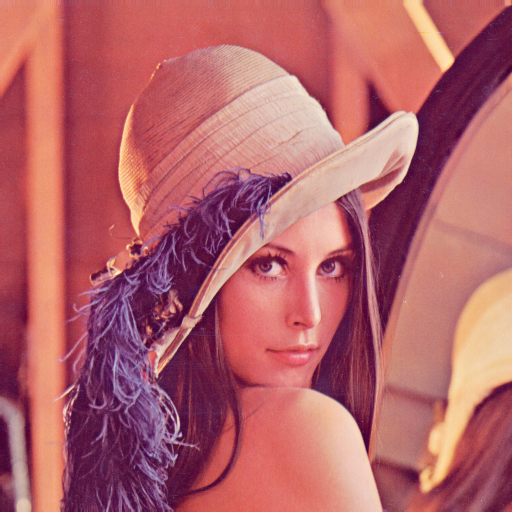
\includegraphics[width=.5\textwidth]{images/lenna}
  \caption{Lena Söderberg}
\end{figure}

        \chapter{Methoden}

In diesem Kapitel werden die angewendeten Techniken und Methoden genau beschrieben. Aufgrund der genauen Beschreibung werden auch mehrere Abschnitte benötigt.

\section{Nichtstun}

In der Regel beginnt man mit dem Nichtstun. Diese sehr einfache Methode kann sofort und von jedem angewandt werden.

\section{Abwarten}

Im zweiten Schritt wird dann gerne abgewartet, ob sich neue Ergebnisse ergeben.
        %!TEX root = advanced.tex

\begin{frame}[fragile]{Zusammenfassung}
  \begin{enumerate}
    \item \LaTeX\ ist sehr gut geeignet für \alert{umfangreiche Dokumente}:
      Es bietet viele Möglichkeiten zur \alert{Strukturierung} und
      \alert{Gliederung}. Ein Dokument kann aus
      \alert{vielen Quelldateien} bestehen.
    \item \alert{\BibTeX} generiert aus einer \alert{Datenbank} in einem eigenen Format
      ein \alert{Literaturverzeichnis}. Die \alert{Zitierweise} kann dabei mit
      \lstinline-\bibliographystyle- eingestellt werden.
    \item Mit \alert{KOMA-Script} können sehr leicht \alert{Papierformate}
      eingestellt, \alert{Satzspiegel}
      berechnet, \alert{Kopf- und Fußzeilen} angepasst werden und vieles
      mehr konfiguriert werden.
    \item \alert{Lies die Anleitung!} Sie ist \emph{sehr} gut.
  \end{enumerate}
\end{frame}

\begin{frame}[fragile]{Zum Weiterlesen}
  \begin{mybib}
    \bibitem{advanced_Kohm}
      Markus Kohm, Jens-Uwe-Morawski.
      \newblock \emph{KOMA-Script},
      \newblock \alt<presentation>{\href{http://mirrors.ctan.org/macros/latex/contrib/koma-script/doc/scrguide.pdf}{\texttt{scrguide.pdf}}}{\url{http://mirrors.ctan.org/macros/latex/contrib/koma-script/doc/scrguide.pdf}}, Dezember 2013.
    \bibitem{Kern}
      Uwe Kern.
      \newblock \emph{Farbspielereien in \LaTeX mit dem xcolor-Paket},
      \newblock Die \TeX nische Komödie 2/2004, S. 35--53,
      \newblock \alt<presentation>{\href{http://jochen-lipps.de/latex/dtk200402.pdf}{\texttt{dtk200402.pdf}}}{\url{http://jochen-lipps.de/latex/dtk200402.pdf}}.
    \bibitem{Schwarz}
      Ulrich Schwarz.
      \newblock \emph{Thmtools Users’ Guide}
      \newblock \alt<presentation>{\href{http://mirrors.ctan.org/macros/latex/exptl/thmtools/thmtools.pdf}{\texttt{thmtools.pdf}}}{\url{http://mirrors.ctan.org/macros/latex/exptl/thmtools/thmtools.pdf}}, April 2014.
  \end{mybib}
\end{frame}

\begin{frame}[fragile]{Zum weiteren Weiterlesen}
  \begin{mybib}
    \bibitem{advanced_Braune}
      Klaus Braune, Joachim und Marion Lammarsch.
      \newblock \emph{\LaTeX: Basissystem, Layout, Formelsatz},
      \newblock Addison-Wesley, Mai 2006.
    \bibitem{advanced_Kopka1}
      Helmut Kopka.
      \newblock \emph{\LaTeX, Band 1: Einführung},
      \newblock Addison-Wesley, März 2002.
    \bibitem{advanced_Kopka2}
      Helmut Kopka.
      \newblock \emph{\LaTeX, Band 2: Ergänzungen},
      \newblock Addison-Wesley, Mai 2002.
  \end{mybib}
\end{frame}

\begin{frame}[fragile]{Zum Weiterlesen für maximal Interessierte}
  \begin{mybib}
    \bibitem{Knuth}
      Donald E. Knuth.
      \newblock \emph{The \TeX book},
      \newblock Addison-Wesley Professional, Januar 1984.
    \bibitem{Victor}
      Victor Eijkhout.
      \newblock \emph{\TeX\ by Topic: A \TeX nician's Reference},
      \newblock Addison-Wesley, Februar 1992.
    \bibitem{Forssmann04}
      Friedrich Forssman, Ralf de Jong.
      \newblock \emph{Detailtypografie: Nachschlagewerk für alle Fragen zu Schrift und Satz}
      \newblock Schmidt (Hermann), Mainz, 4. Auflage, Juni 2004.
    \bibitem{Forssmann05}
      Friedrich Forssman, Hans Peter Willberg.
      \newblock \emph{Lesetypografie}
      \newblock Verlag Hermann Schmidt, Mainz, Oktober 2005.
  \end{mybib}
\end{frame}

      \end{document}
    \end{lstlisting}
  \end{columns}
\end{frame}

\begin{frame}[fragile]{Befehle für modulare Struktur}
  \begin{tabular}{rL{6cm}}
    \lstinline-\input- & Inhalt der Datei einfügen. \\[1ex]
    \lstinline-\include- & Inhalt der Datei einfügen und \newline
      Seitenumbrüche davor und dahinter.\\[1ex]
    \lstinline-\includeonly- & Liste der von \lstinline-\include- \newline
      berücksichtigten Dateien.\\
  \end{tabular}
\end{frame}

\livecoding{Modulare Dokumente in der Praxis}

